\chapter{Конструкторский раздел}

В рамках данного раздела приведены основные требования к программному обеспечению (далее -- ПО), описаны используемые структуры данных и алгоритмы.

\section{Требования к программному обеспечению}

Разрабатываемое ПО должно предоставлять следующие возможности:

\begin{itemize}[label=---]
	\item визуальное отображение сцены с объектами;

	\item добавление моделей из числа примитивов и их удаление;
	\item загрузка сцены из файла;
	\item выбор конкретной модели или её составляющей части (вершины, ребра или грани);
	\item преобразование конкретной модели или её составляющей части.
\end{itemize}

Более того, модели на сцене должны состоять только из треугольных граней.
	
\section{Основные структуры данных}

Для формализации общего алгоритма синтеза изображения необходимо определить использующиеся в программе структуры данных. Ниже приведены основные структуры данных и их составляющие.

\begin{enumerate}
	\item \textbf{Сцена.} Состоит из
	\begin{itemize}[label=---]
		\item списка моделей,
		\item списка источников света,
		\item камеры.
	\end{itemize}
	\item \textbf{Модель.} Состоит из
	\begin{itemize}[label=---]
		\item названия,
		\item списка вершин,
		\item списка ребер,
		\item списка граней,
		\item вершины, определяющей центр модели.
	\end{itemize}
	\item \textbf{Источник света.} Состоит из
	\begin{itemize}[label=---]
		\item названия,
		\item вершины, определяющей местоположение источника,
		\item интенсивности источника.
	\end{itemize}
	\item \textbf{Камера.} Состоит из
	\begin{itemize}[label=---]
		\item вершины, определяющей местоположение источника,
		\item вершины, к которой направлен объектив камеры.
	\end{itemize}
	\item \textbf{Вершина.} Состоит из
	\begin{itemize}[label=---]
		\item начальных ее координат,
		\item матрицы трансформации.
	\end{itemize}
	\item \textbf{Ребро.} Состоит из
	\begin{itemize}[label=---]
		\item начальной вершины ребра,
		\item конечной вершины ребра.
	\end{itemize}
	\item \textbf{Грань.} Состоит из
	\begin{itemize}[label=---]
		\item списка принадлежащих ей вершин,
		\item списка принадлежащих ей ребер.
	\end{itemize}
\end{enumerate}

\section{Алгоритм визуального отображения сцены}

Схема общего алгоритма визуального отображения сцены изображена на рисунке \ref{fig:rendering}. 

Схема алгоритма обработки грани в несколько потоков представлена на рисунке \ref{fig:face}, а схема обработки обрамляющего прямоугольника грани -- на рисунке \ref{fig:framing_rect}.

\begin{figure}[h]
	\centering
	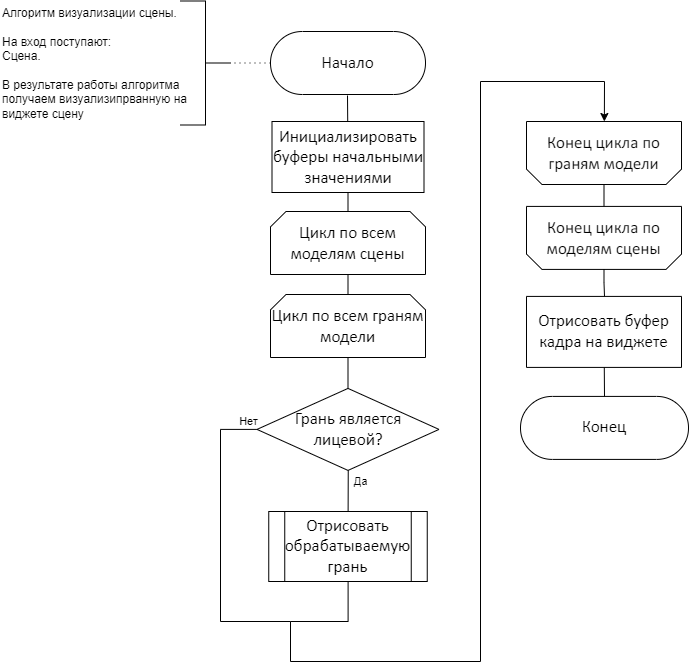
\includegraphics[scale=0.67]{inc/img/rendering.png}
	\caption{Алгоритм визуализации сцены}
	\label{fig:rendering}
\end{figure} 

\begin{figure}[h]
	\centering
	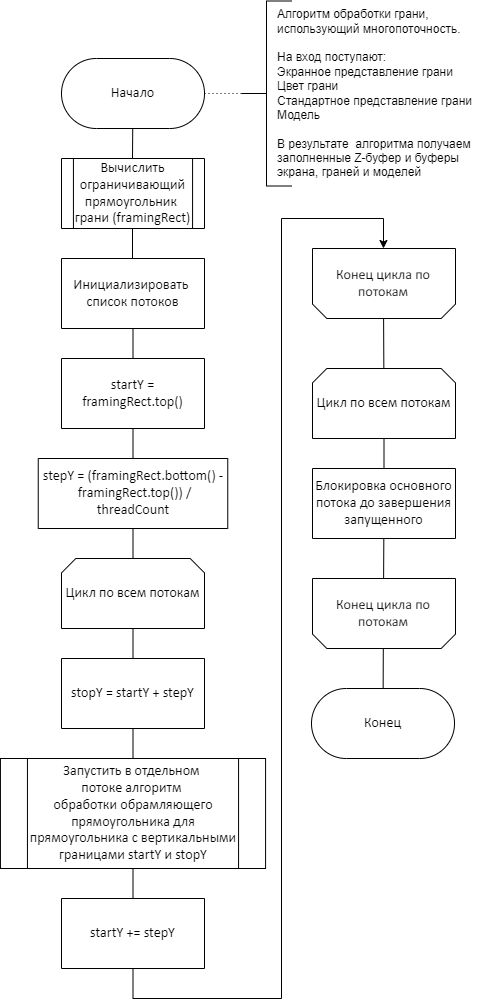
\includegraphics[scale=0.6]{inc/img/face.png}
	\caption{Алгоритм обработки грани с использованием многопоточности}
	\label{fig:face}
\end{figure} 

\begin{figure}[h]
	\centering
	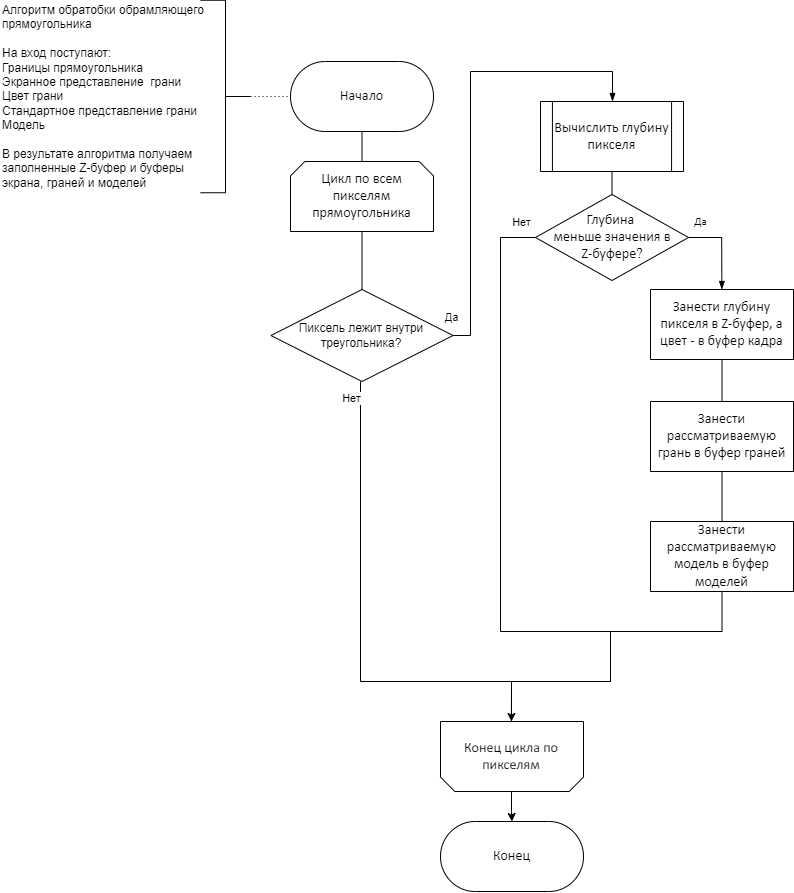
\includegraphics[scale=0.57]{inc/img/framing_rect.png}
	\caption{Алгоритм обработки обрамляющего прямоугольника}
	\label{fig:framing_rect}
\end{figure} 

\clearpage

\section{Поиск экранных координат вершины}

В рамках алгоритма обработки грани необходимо вычислять экранные координаты вершин грани.

Поиск экранных координат вершины предполагает последовательное применение к начальным ее координатам следующих преобразований:
\begin{enumerate}
	\item аффинных преобразований;
	\item преобразований камеры;
	\item перспективных преобразований, если включена соответствующая опция.
\end{enumerate}

\subsection{Аффинные преобразования}

Первым этапом получения экранных координат вершины является применение к ней аффинных преобразований. Это преобразование осуществляется путем умножения матрицы трансформации вершины на матрицу соответствующего аффинного преобразования.

В данном проекте над вершиной можно произвести следующие аффинные преобразования:

\subsubsection*{Перенос.}

Перенос в трехмерном пространстве задается значениями переноса вдоль осей OX, OY, OZ - $dx$, $dy$, $dz$ соответственно. Матрица переноса имеет вид:

\begin{equation}
	\begin{pmatrix}
		1  & 0  & 0  & 0 \\
		0  & 1  & 0  & 0 \\
		0  & 0  & 1  & 0 \\
		dx & dy & dz & 1
	\end{pmatrix}
\end{equation}

\subsubsection*{Поворот.}
	
Поворот описывается углом $\theta$ и осью вращения. Матрицы поворота имеют вид:

\begin{itemize}[label=---]
	\item Вокруг оси OX:
	\begin{equation}
		\begin{pmatrix}
			1 & 0             & 0            & 0 \\
			0 & cos\ \theta   & \sin{\theta} & 0 \\
			0 & -\sin{\theta} & \cos{\theta} & 0 \\
			0 & 0             & 0            & 1
		\end{pmatrix}
	\end{equation}

	\item Вокруг оси OY:
	\begin{equation}
		\begin{pmatrix}
			\cos{\theta} & 0 & -\sin{\theta} & 0 \\
			0            & 1 & 0             & 0 \\
			\sin{\theta} & 0 & \cos{\theta}  & 0 \\
			0            & 0 & 0             & 1
		\end{pmatrix}
	\end{equation}

	\item Вокруг оси OZ:
	\begin{equation}
		\begin{pmatrix}
			\cos{\theta}  & \sin{\theta} & 0 & 0 \\
			-\sin{\theta} & \cos{\theta} & 0 & 0 \\
			0             & 0            & 1 & 0 \\
			0             & 0            & 0 & 1
		\end{pmatrix}
	\end{equation}
\end{itemize}

\subsubsection*{Масштабирование.}
	
Масштабирование в трехмерном пространстве задается значениями масштабирования вдоль осей OX, OY, OZ - $kx$, $ky$, $kz$ соответственно. Матрица масштабирования имеет вид:

\begin{equation}
	\begin{pmatrix}
		kx & 0  & 0  & 0 \\
		0  & ky & 0  & 0 \\
		0  & 0  & kz & 0 \\
		0  & 0  & 0  & 1
	\end{pmatrix}
\end{equation}
	
При этом важно заметить, что перед применением преобразований поворота и масштабирования необходимо предварительно осуществить перенос вершины так, чтобы центр соответствующего преобразования совпал с центром координат.

\subsection{Приведение к пространству камеры}

Приведение к пространству камеры производится путем умножения матрицы трансформации вершины на матрицу преобразования камеры. При этом стоит учитывать, что над камерой возможно осуществления лишь 2 вида преобразования: перенос и поворот, которые производятся над вершиной, задающей местоположение камеры.

\subsection{Проецирование вершины}

После перехода в пространство камеры необходимо спроецировать вершину на картинную плоскость. В данном курсовом проекте используется перспективная и ортогональная проекции.

Для получения ортогональной проекции вершины не требуется каких-либо дополнительных преобразований.

В моем проекте используется одноточечная перспективная проекция \cite{rogers_math}. Для получения перспективной проекции вершины необходимо умножить полученную на предыдущих шагах матрицу ее трансформации на матрицу одноточечной перспективной проекции:

\begin{equation}
	\begin{pmatrix}
		1 & 0 & 0 & 0 \\
		0 & 1 & 0 & 0 \\
		0 & 0 & 1 & r \\
		0 & 0 & 0 & 1
	\end{pmatrix}, \text{где } r=\frac{1}{F},F \text{-- фокус}
\end{equation}

\subsection{Определение нелицевых граней}

С помощью отбрасывания нелицевых граней моделей при построении изображения можно существенно сократить временные затраты, так как грани, невидимые по отношению к камере, визуализироваться не будут.

Пусть
$\bar{N}$ --- вектор внешней нормали к грани модели,
$\bar{V}$ – вектор от камеры до любой точки грани.

Для определения видимости грани используется формула:

\begin{equation}
	(\bar{N},\bar{V})=
	\begin{cases}
		\geq 0, & \text{если грань невидима} \\
		< 0,   & \text{если грань видима}
	\end{cases}
\end{equation}

\section{Вычисление глубины пикселя}

В рамках алгоритма обработки обрамляющего прямоугольника требуется определить, лежит ли пиксель внутри треугольника, задающего грань. И, если лежит, вычислить его глубину.

Для решения этих задач для каждого пикселя ограничивающего прямоугольника находятся его барицентрические координаты относительно вершин треугольной грани.

Пусть $A$, $B$, $C$ – вершины полигона, $P$ – пиксель внутри ограничивающего прямоугольника.

Площадь треугольника можно найти по следующей формуле:

\begin{equation}
	square=\left(A_y-C_y\right)\cdot\left(B_x-C_x\right)+\left(B_y-C_y\right)\cdot\left(C_x-A_x\right)
\end{equation}

Тогда барицентрические координаты пикселя равны:

\begin{equation}
	\alpha=\frac{\left(P_y-C_y\right)\cdot\left(B_x-C_x\right)+\left(B_y-C_y\right)\cdot\left(C_x-P_x\right)}{square}
\end{equation}	

\begin{equation}
	\beta=\frac{\left(P_y-A_y\right)\cdot\left(C_x-A_x\right)+\left(C_y-A_y\right)\cdot\left(A_x-P_x\right)}{square}
\end{equation}

\begin{equation}
	\gamma=1-\ \alpha-\ \beta
\end{equation}

В случае, если хоть одна из барицентрических координат отрицательна, то пиксель лежит вне полигона. Если пиксель лежит внутри треугольника, то найти значение его глубины можно по следующей формуле:

\begin{equation}
	z=\frac{1}{\frac{\alpha}{A_z}+\frac{\beta}{B_z}+\frac{\gamma}{C_z}}
\end{equation}

\section{Простая модель освещения}

В простом методе освещения цвет пикселя рассчитывается по закону Ламберта. При этом положение наблюдателя не имеет значения, т.к. диффузно отраженный свет рассеивается равномерно по всем направлениям (рисунок \ref{fig:simple_light}).

\begin{figure}[h]
	\centering
	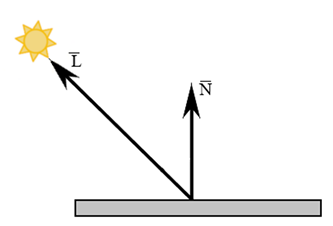
\includegraphics[scale=0.8]{inc/img/simple_light.png}
	\caption{Простая модель освещения}
	\label{fig:simple_light}
\end{figure} 

Пусть 
$ I $ -- результирующая интенсивность света в точке,
$ \bar{L} $ -- вектор от точки до источника,
$ \bar{N} $ -- вектор нормали,
$ I_0 $ -- интенсивность источника,
$ k_d $ -- коэффициент диффузного освещения.

Формула расчёта интенсивности имеет следующий вид:

\begin{equation}
	I=I_0 \cdot k_d \cdot \left(\bar{L},\bar{N}\right)
\end{equation}

\section{Алгоритм выбора составляющей части модели}

Общая схема алгоритма выбора составляющей части модели изображена на рисунке \ref{fig:selection}.

\begin{figure}[h]
	\centering
	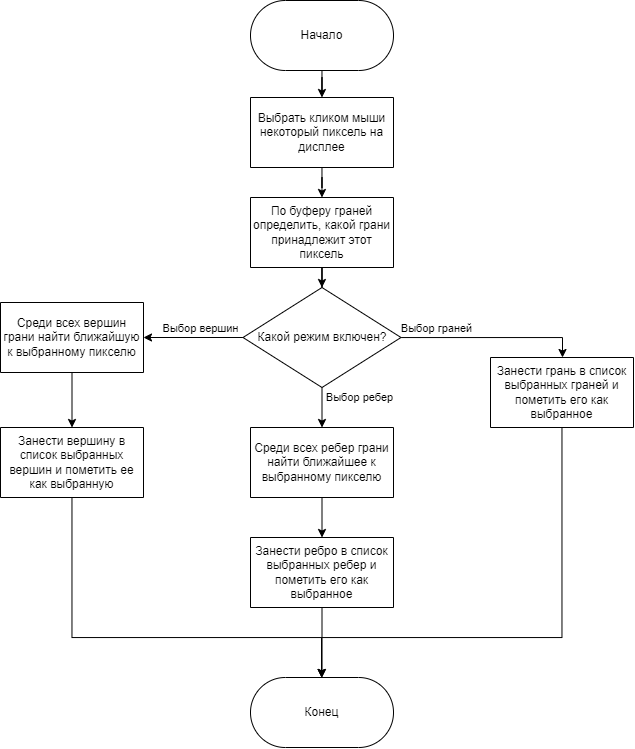
\includegraphics[scale=0.7]{inc/img/selection.png}
	\caption{Алгоритм выбора составляющей части модели}
	\label{fig:selection}
\end{figure} 



